\documentclass[a4paper,11pt]{article}
\usepackage[T1]{fontenc}
\usepackage[u  tf8]{inputenc}
\usepackage{mathtools}
\usepackage{mathrsfs}
\usepackage{bm}
\usepackage{amsfonts}
\usepackage[dvipsnames]{xcolor}
% \usepackage{cleveref}
\usepackage[normalem]{ulem}
\usepackage{graphicx}
\usepackage{fullpage}
\usepackage[margin=1in]{geometry}
\usepackage{natbib}
\usepackage{amsmath}
%\usepackage{float}
%\usepackage{subcaption}
%\usepackage{multirow} 
\usepackage[colorlinks = true,urlcolor=blue]{hyperref}
%\usepackage{bibunits}
%\usepackage{csvsimple}
%\usepackage[superscript,biblabel]{cite}
\usepackage{verbatim}
\usepackage{graphicx}
\graphicspath{ {final_images/} }
\usepackage{subfig}
%\usepackage{subcaption}

\newcommand{\jb}[1]{{\color{blue} (#1)} }
\begin{document}

\title{\vspace{-2cm}
  Title here
}
\author{Kyelee Ruth Fitts}
\maketitle


\subsection*{Abstract}

\subsection*{Introduction}

The diversity of life on Earth is due in large part to the
adaptation of organisms to their varying environments. We now know that
adaptation has a large genetic basis. Thus, understanding how and why such
genetic variation occurs is a major goal of evolutionary
biology. Quantifying genetic adaptation is an important aim of population
geneticists, and to this end finding methods to detect signals of
selection within the genome is of particular interest. Change in the
mean phenotype of a population over time can be attributed to many causes including genetic
drift or population migration, so detecting signals of selection in
particular is no trivial task.

Until recently, the population genetic methods to detect recent adaptation have been limited to
large-effect alleles, when in fact numerous phenotypic traits of interest
are affected by many different loci across the genome. Understanding
how to find signals of natural selection for such polygenic traits has been
the subject of much study in recent years. Increased computational
capabilities have given us the tools to be able to evaluate the effects
of many thousands of loci on a trait, allowing us to evaluate
selection in highly polygenic traits, such as height. One of the most
important tools developed are Genome-Wide Association Studies (GWAS)
which determine which loci across the genome have significant effects
on a certain polygenic trait \cite{gwasoverview}. The effect sizes
measured by GWAS for loci on a certain polygenic trait are often
denoted $\alpha$.

We can express the polygenic phenotype of individuals in a population
as the weighted sum of genotypes with additive effect sizes
$\alpha$. This generalizes to population means, where the mean
population phenotype is the weighted sum of effect sizes and frequency
of the allele ($p$) at each significant locus ($l$). \jb{cite--
  Gillepsie? for additive model} 

\begin{equation}
  \sum_l{\alpha_lp_l}
\end{equation}

The additive effect size, then, is key to relating the genotypes of
the many loci contributing to the phenotype of interest with the
phenotype itself-- as shown below, it also plays a key role in statistical tests for
polygenic adaptaion. Understanding how $\alpha$ can be
affected by other factors is essential for ensuring that these
statistical tests remain as unbiased as possible. 

Dominance is one such phenomenon that we hypothesize has a non-trivial
effect on $\alpha$. Dominance in population genetics refers to when the effect of one
allele depends on the presence of another allele at the locus. We can account for
the effect of dominance in the effect size by parametrizing $\alpha$
in terms of the homozygous effect size (A), or effect size of the most frequent homozygote, and the
dominance deviation (D), which is the difference in effect size for the heterozygote
deviating from $\frac{1}{2}$ of the homozygous effect size \jb{cite Gillepsie?}:

\begin{equation}  
  \alpha_\ell = \frac{1}{2} A_\ell + D_\ell\left(1-2p_{1\ell}\right).
  \label{alpha}
\end{equation}

In particular, directional dominance is when alleles with a postive effect
size on the trait are systematically dominant and alleles with a
negative effect size on the trait are systematically negative. In
terms of \eqref{alpha}, this means that the signs of A and D are the
correlated for a large number of loci. We hypothesized that
directional dominance is problematic in tests of polygenic adaptation
because the effect size we estimate in the presence of directional
dominance depends on how the allele frequency $p$ has changed in the
recent past. In particular, recessive alleles which have decreased in frequency
in the recent past will tend to have larger effect sizes, as shown in
Figure 1 in the supplement. Notice that when there is no dominance,
$\alpha$ is constant, but in the presence of directional dominance
(positive A and D) for alleles with lower frequency will have a higher
effect size. 

Given the hypothesized effect that directional dominance has on
$\alpha$, we suspect that directional dominance will bias statistical
tests of polygenic adaptation. We give a short overview of such tests
below.  

Wright first introduced the parameter $F_{st}$ as a measure comparing
the genetic variation of an allele at a specific site in a subpopulation to that of the entire population
\cite{Fst}. Lewontin and Krakauer, using this parameter developed a
novel statistical test based on the fact
that under no selection, the expected $F_{st}$ at a given site will be the same
as the population $F_{st}$. Further, they concluded that the
distribution of $F_{st}$ across all sites will be chi-squared
$F_{st}$ \cite{firstseltest}. The natural conclusion is that sites
with statistically different $F_{st}$ values are candidates for loci
that have been acted upon by selection. These conclusions were extended by Spitze, who coined the
parameter $Q_{st}$ as a measure of how the variation of all loci
contributing to a phenotype of a subpopulation compares to that of the entire
population \cite{Qst}. Essentially, $Q_{st}$ is analogous to $F_{st}$,
except that instead of looking at the variation of one allele at a
locus, it measures the ratio of the variation of all loci contributing to a
phenotype within a subpopulation to that of the entire population. These early tests for selection utilized the ratio
$\frac{Q_{st}}{F_{st}}$ as a test statistic for detecting signals of
selection, where $F_{st} = Q_{st}$ is the null model, where no
selection occurs.

Much later, Berg and Coop introduced a comprehensive test statistic,
called $Q_x$, based on these central ideas to test
for selection \cite{berg}. This statistic depends on $F_{st}$ and
a generalized analogy to $Q_{st}$, expressed in terms of $\alpha$ and
the allele frequencies $p$ over loci $l$ and $l'$, summed over
populations $m$. $V_a$ is the additive genetic variance of the entire
population, and $\overline{p}_l$ is the mean frequency.

\begin{equation} \label{Qxraw}
  Q_X = \frac{1}{V_A F_{ST}} \sum_{m=1}^M \sum_{\ell=1}^L \sum_{\ell\prime=1}^L \alpha_{\ell} \alpha_{\ell^{\prime}}\left(p_{m\ell} - \overline{p}_\ell \right)\left(p_{m \ell\prime} - \overline{p}_{\ell\prime}\right)
\end{equation}


The distribution of this statistic is expected to be chi-squared. Notice that the additive effect size $\alpha$ is the weighting factor for loci in the
expression for $Q_x$. 

In the presence of directional dominance, we hypothesized a bias in
tests for polygenic adaptation that depends on $\alpha$. Alleles which are systematically dominant and which have recently increased in
frequency (large p, positive D) will tend to have smaller effect sizes, while
alleles which are recessive which have recently decreased in frequency
(small p, negative D) will tend to have larger effect sizes. In the
latter case, the test for polygenic selection advanced by Berg and Coop
\eqref{Qxraw} will tend to make false positive judgements for
selection, because the statistic will be calculated over alleles which
do not actually increase the effect size.

Height is one polygenic trait with many well-defined signficant
alleles via GWAS \cite{heightselection}. It has also been shown to exhibit
directional dominance \cite{heightdirectdom}. We aim to quantify the
hypothesized bias, first with simulated populations, then with height genotype data from the UK Biobank.



\subsection*{Theory/Methods}

Using the expression for the test statistic $Q_x$ \eqref{Qxraw}, we
can substitute the expression for $\alpha$ \eqref{alpha} and manipulate
the expression algebraically to derive the following expansion for the
test statistic, in terms of the homozygous effect (A)  and the dominance
deviation (D):

\begin{equation}
  \begin{split}
  \sum^L_{l=1}( \frac{1}{2}A_l(p_{1l}-\epsilon_l))^2+\sum^L_{l=1}\sum^L_{
    l \neq l'}(\frac{1}{4}A_l(p_{1l}-\epsilon_{l})A_{l'}(p_{1l'}-\epsilon_{l'}))
  \\
  +\sum^L_{l=1}A_lD_l(1-2p_{1l})(p_{1l}-\epsilon_l)^2 +
  \sum^L_{l=1}\sum^L_{l \neq
    l'}(\frac{1}{2}A_lD_{l'}(1-2_{p1l'})(p_{1l}-\epsilon_l)(p_{1l'}-\epsilon_{l'}) \\
  + \frac{1}{2}D_lA_{l'}(1-2_{p1l})(p_{1l}-\epsilon_l)(p_{1l'}-\epsilon_{l'})) \\
   + \sum^L_{l=1} (D_l(1-2p_l)(p_{1l}-\epsilon_{1}))^2
   + \sum^L_{l=1}\sum^L_{l \neq
     l'}D_{l}(1-2p_{l})(p_{1l}-\epsilon_{1})D_{l'}(1-2p_{l'})(p_{1l'}-\epsilon_{l'}) \label{expansion}
  \end{split}
\end{equation}

We can loosly consider the single summation terms to be variances
corresponding to the expansion of additive effects multiplied by
additive effects, additive times dominance, and dominance times
dominance, and the double summation terms as covariances of these
quantities. We expect the inflation of the test statistic due to
dominance effects to come from the last two terms. Note that when
dominance is not present ($D=0$) the expansion reduces to the
expression Berg and Coop present when $\alpha$ is treated as a constant
\cite{berg}.

Using this expansion, we have created simulations to characterize our
hypothesized dominance bias. We used simulated populations
under a couple of assumptions: first, that the values of the dominance
deviations and homozygous effects are constant throughout the
population. While this is not true in general, \jb{why is this
  justified? cite??} Second, that $F_{st}$ for these simulated approximations
can be roughly estimated by the number of generations elapsed over the
population size. Third, that the distribution of allele frequencies after
one generation can be approximated by a normal distribution centered
at the ancestral frequency with variance
$F_{st}*\epsilon*(1-\epsilon)$ where $\epsilon$ is the ancestral
frequency. \jb{CITE THESE ASSUMPTIONS???}

All simulations were performed in R. 

\subsection*{Results/Discussion}
Simulations of the expansion \eqref{expansion} were performed with
population size $10000$ over 100 generations, starting at an ancestral
frequency of 0.5, an homozygous effect size of 0.5, and a dominance
deviation value of 0. The distribution of $Q_x$ was simulated under
these conditions for 1000 replicates. The distribution was roughly
chi-squared, as expected, with mean of 0.99 and variance of 2.2.  


% \subsection*{Supplement}
% \begin{table}[ht]
% \centering
% \begin{tabular}{ p{8cm}p{8cm} }
% 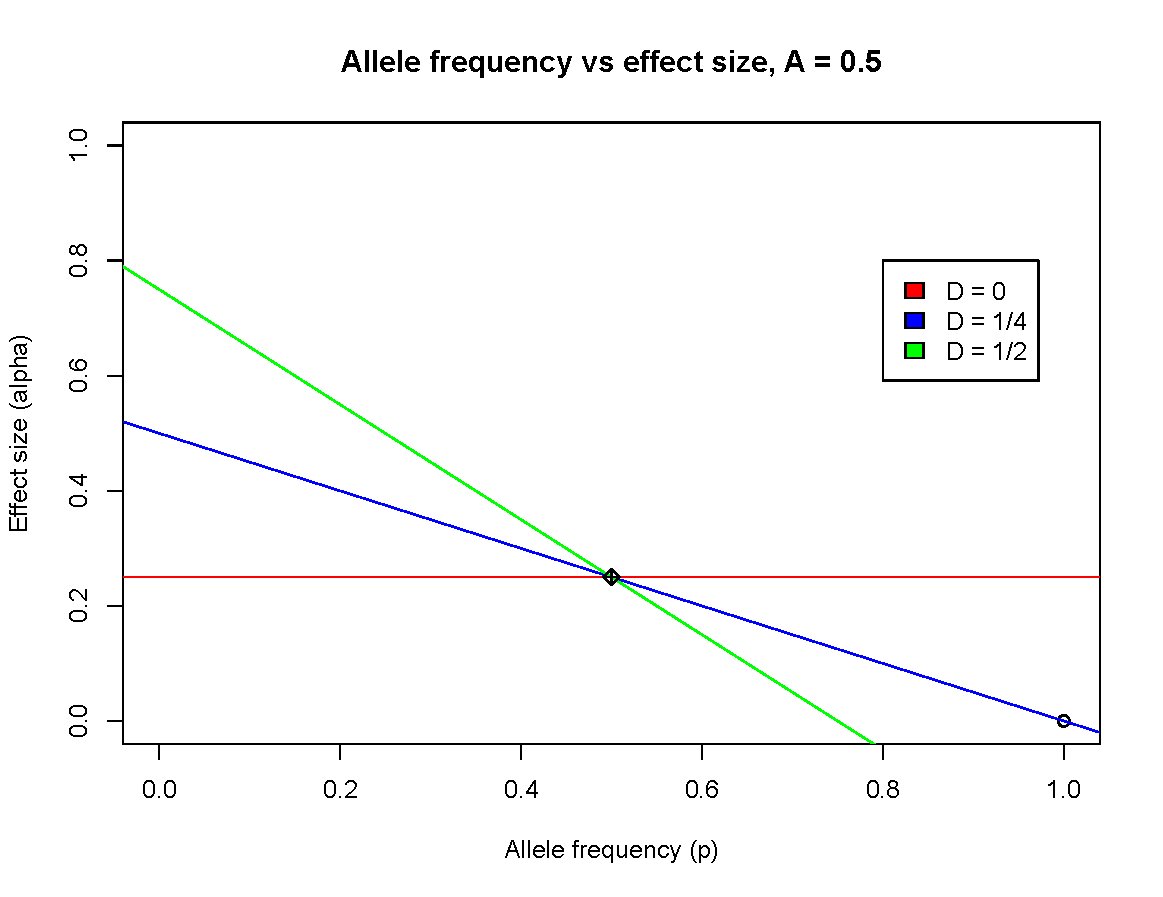
\includegraphics[width=90mm]{alpha} \caption*{Fig. 1: Effect sizes for various
%   dominance deviation values under directional dominance}
%   &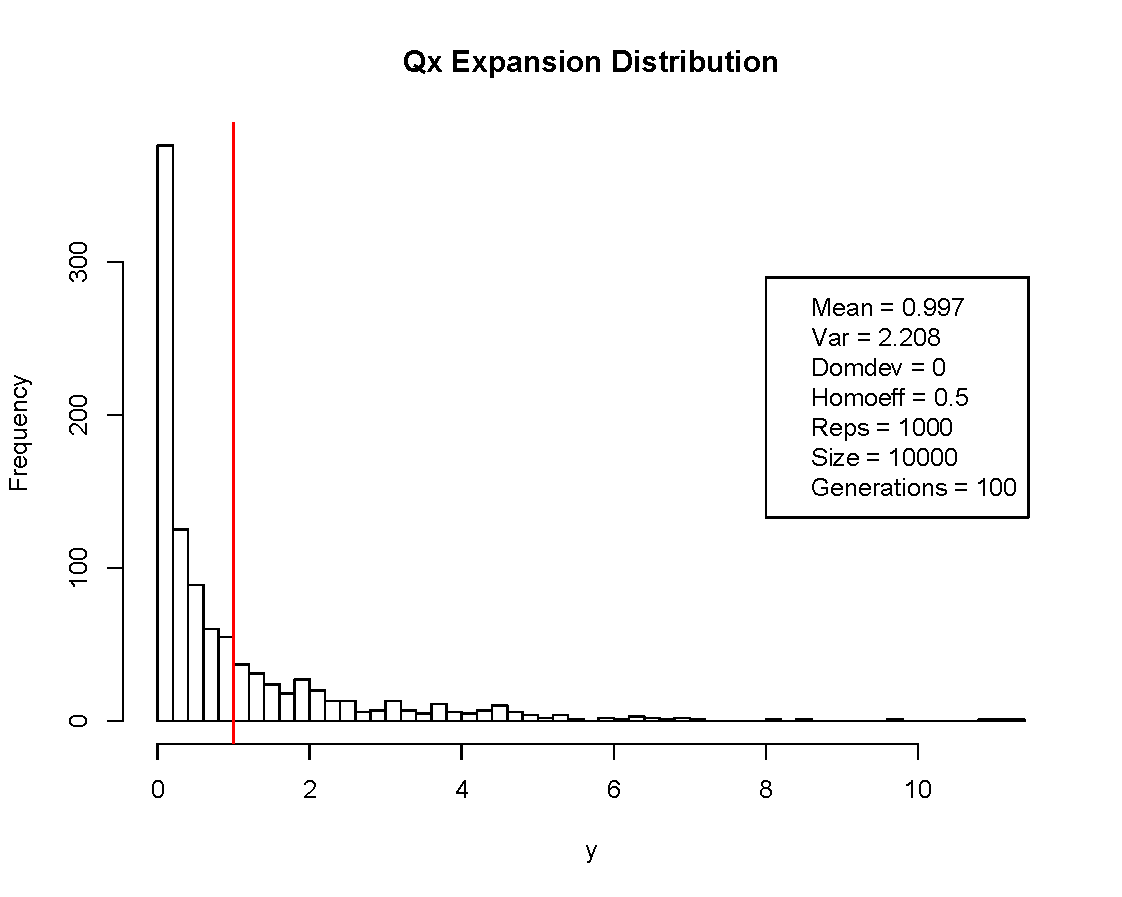
\includegraphics[width=90mm]{Qxexpdist} \caption*{Fig. 2: $Q_x$
%     Expansion Distribution} \\
% \newline
% 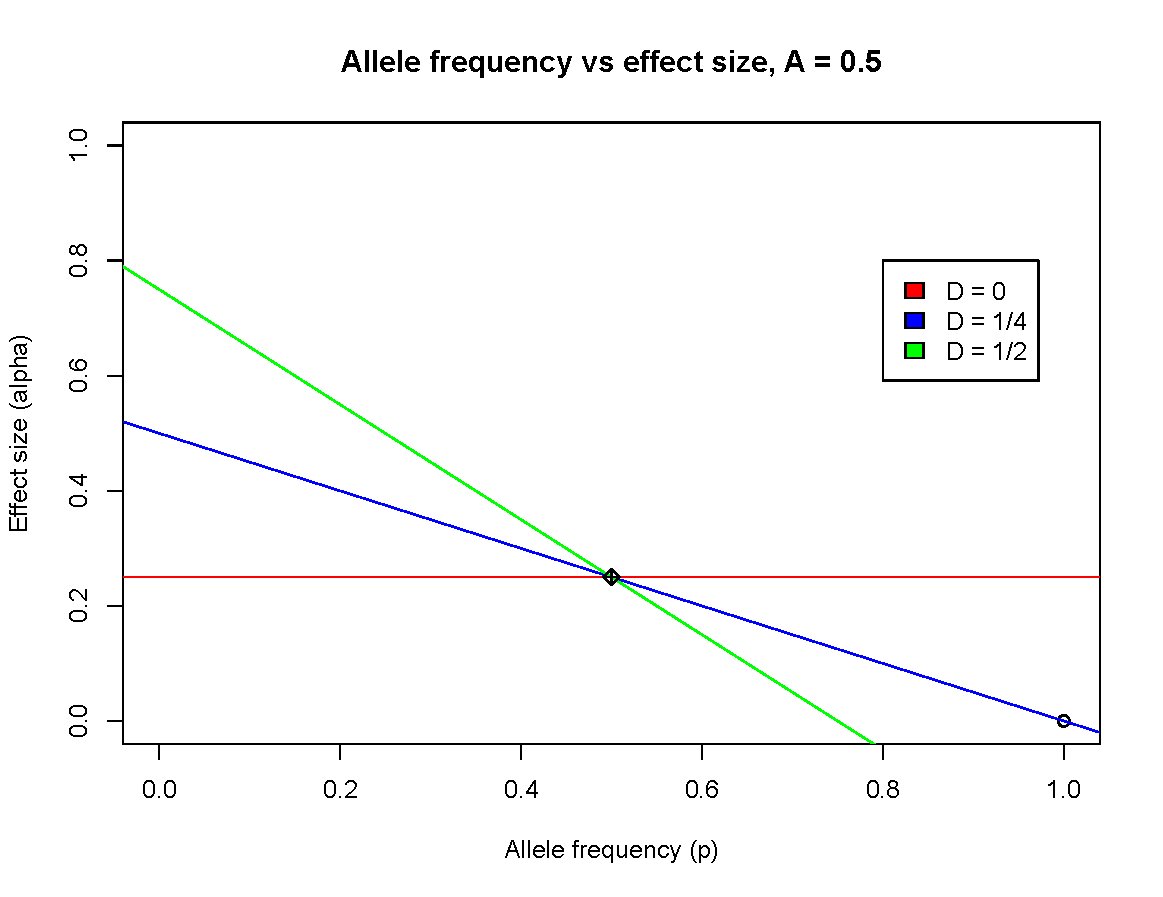
\includegraphics[width=90mm]{alpha}
%   &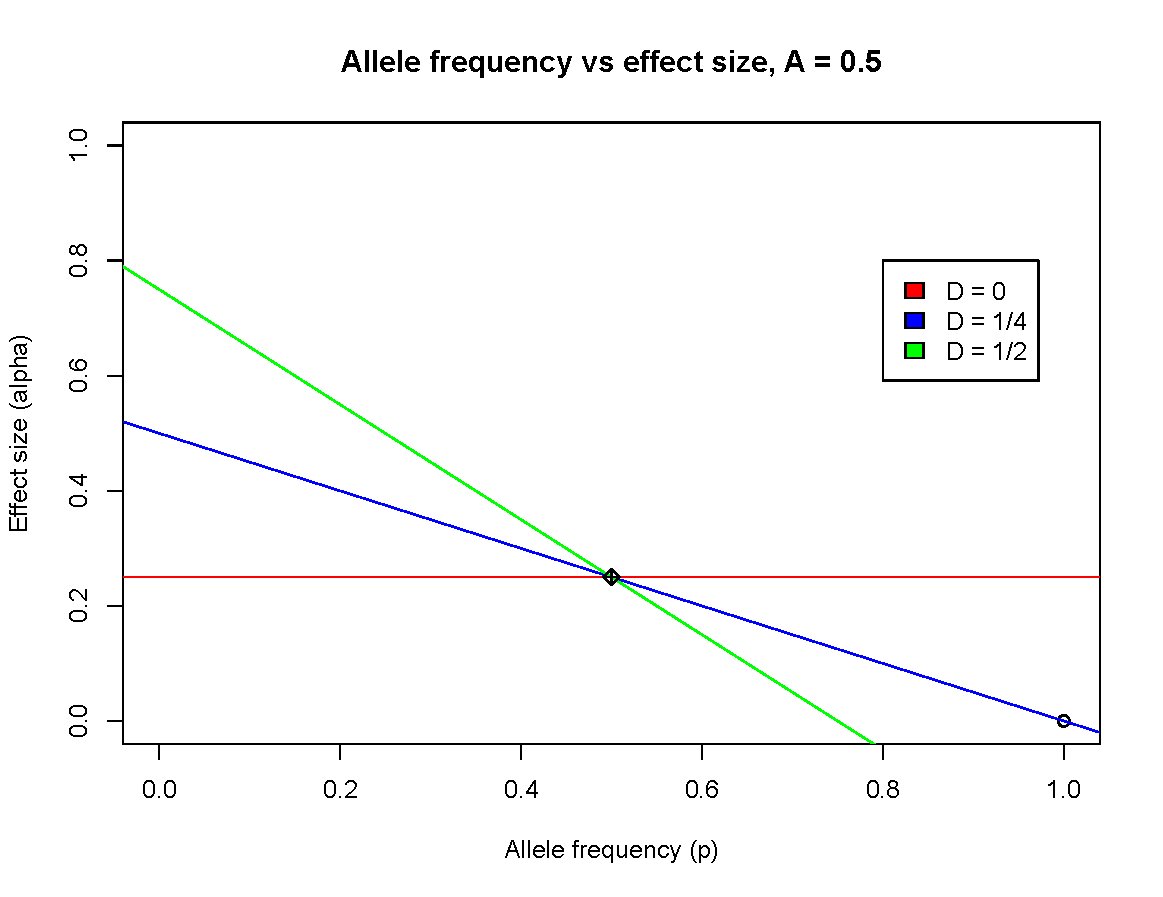
\includegraphics[width=90mm]{alpha}\\
% \end{tabular}
% \end{table}

\pagebreak

\bibliography{works_cited}
\bibliographystyle{plain}






\end{document}
